\documentclass{sig-alternate-05-2015}

% Do not include ISBN and DOI info
\makeatletter
\def\@copyrightspace{\relax}
\makeatother

\begin{document}

\title{CS 211 course project proposal: \\Remote access to OpenWRT}

\numberofauthors{3}

\author{
\alignauthor
Zhehao Wang \\
  \email{zhehao@cs.ucla.edu}
% 2nd. author
\alignauthor
Haitao Zhang \\
  \email{haitao@cs.ucla.edu}
% 3rd. author
\alignauthor 
Jeffrey Chen
}

\maketitle
\section{literature survey}

\subsection{What is OpenWrt}
OpenWrt \cite{fainelli2008openwrt, kim2014implementation} is a Busybox/Linux based embedded platform which is developed following GPL license. It minimizes its own functions so that it fits for lots of memory constrained devices. Specifically, it builds the appropriate toolchain for devices, compiles appropriate kernel with patched and options, as well as provides software as IPKG packages.

\subsection{OpenWrt System Structure}
OpenWrt System Structure covers four aspects: directory structure, packages and external repositories, toolchain, and software architecture.

There are four key directories in the base: tools, toolchain, package and target.
Tools and toolchain refer to common tools which will be used to build the firmware image, the compiler, and the C library.

In an OpenWrt, almost all the packages are .ipk files. Users can choose what packages to install and what packages to uninstall based on their specific needs. Packages are either part of the main trunk or maintained out of the main trunk. For the second case, packages can be maintained by the package feeds system.

To compile the program for a particular architecture, the toolchain will be automatically created by the OpenWrt system during the cross-compilation process. That will simplify developers tasks. However, when there are needs to create toolchain by hand, OpenWrt also provides an easy way to configure the arguments.

The following figure \ref{OpenWrt:stack} shows the software stack of OpenWrt. We can see that the common embedded Linux tools such as uClibc, busybox, shell interpreter are used by OpenWrt, so there is no need to learn some complex things.

\begin{figure}
	\centering
	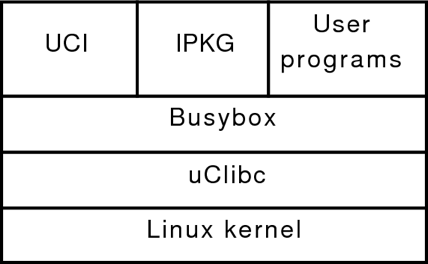
\includegraphics[width=0.4\textwidth]{stack.png}
	\caption{the software stack of OpenWrt}
	\label{OpenWrt:stack}
\end{figure}

\subsection{How to Develop With OpenWrt}

\subsection{Web-based Access to OpenWrt}

\section{Design and implementation \\ roadmap}

This section covers the functional components of the application, which are organized into three major categories.

\begin{itemize}

\item
\textbf{Network configuration} covers common functionalities in configuration tools that often come with commercial APs. These configurations include, but may not be limited to, managing network interfaces, DHCP and DNS settings, static routes, and firewall.

\item
\textbf{System configuration} provides interface to customize the OpenWRT box. Common adminstration functions include: system and user configuration (setting device adminstrator password, creating system backup image and restoring system from backup image, generating user SSH keys, etc), software management (installing and configuring software packages), task management (managing scheduled task and startup task)

\item
\textbf{Status/Statistics visualization} offers a mobile-phone friendly view of the system status (Firmware and kernel version, uptime, current time; CPU and memory usage, currently running processes, and system and kernel log) and network-related status (Interface, route, and firewall status, etc). The visualization component could provide realtime graphs of system load and traffic statistics, for example, traffic per interface and traffic per transport layer connection.

\end{itemize}

The design and implementation effort will be organized by the three function categories, with approximately two weeks dedicated to each.

\section{Timeline}

A rough timeline for the project is given in table \ref{table:timeline}

\begin{table}[h]
\centering
\caption{Project timeline}
\label{table:timeline}
\begin{tabular}{p{3cm}|p{5cm}} \hline
Week No. & Task \\ \hline
5, 6 (first half) & Implement status/statistics visualization module \\ \hline
6 (second half), 7 & Implement network configuration module \\ \hline
8, 9 (first half) & Implement system configuration module \\ \hline
9 (second half), 10 & Prepare final report and presentation \\
\hline\end{tabular}
\end{table}

\end{document}